%!TEX root = ../main.tex

\section{Results}

\begin{frame}
\frametitle{A smooth problem: Moffatt eddies inside a wedge}
\centering
\begin{figure}
	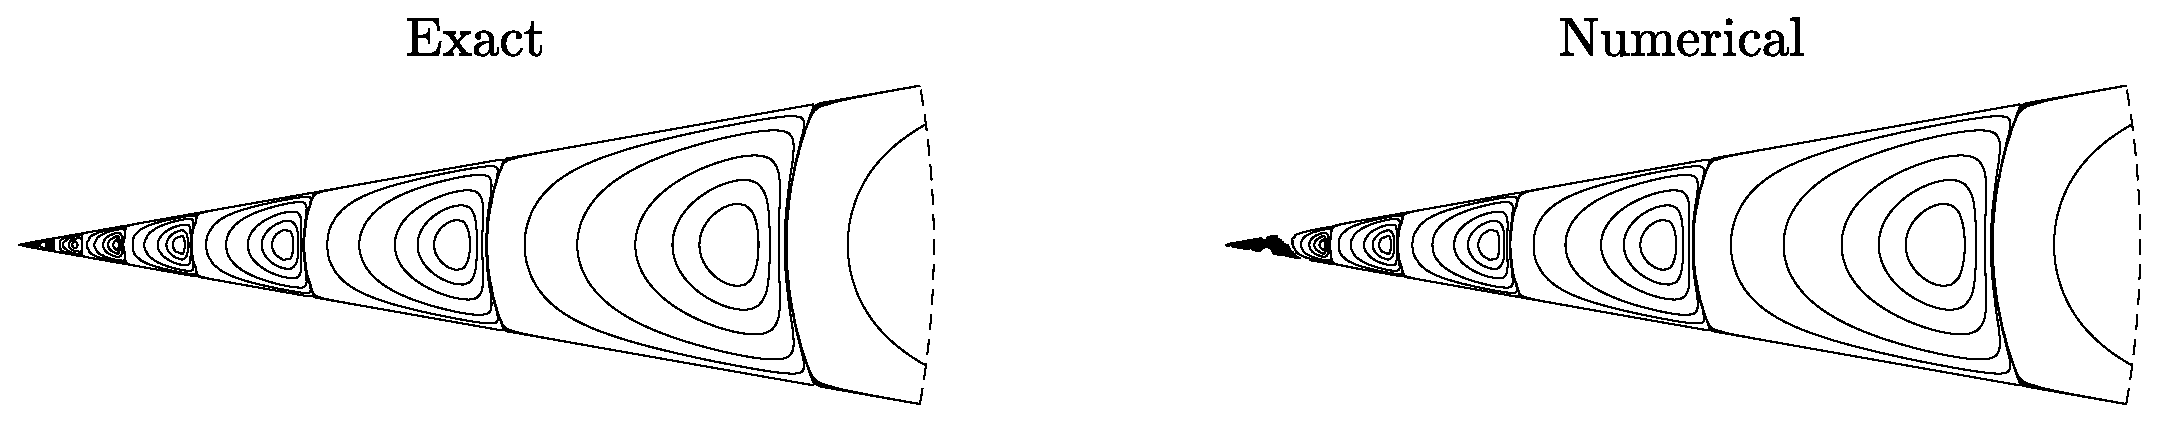
\includegraphics[width=\linewidth]{Figures/moff_psi}
	
	\vfill
	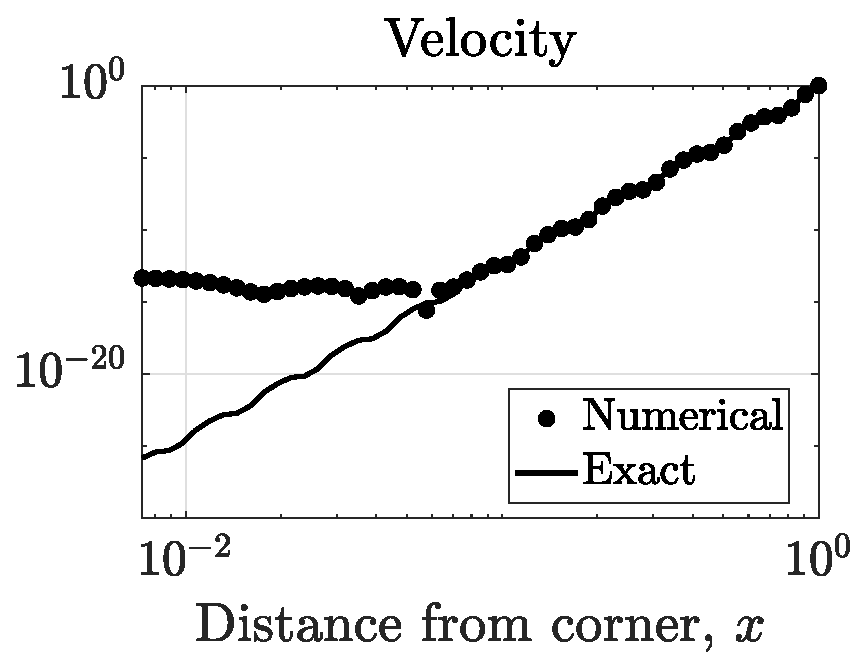
\includegraphics[height=0.3\linewidth]{Figures/moff_vel}
	\hfill
	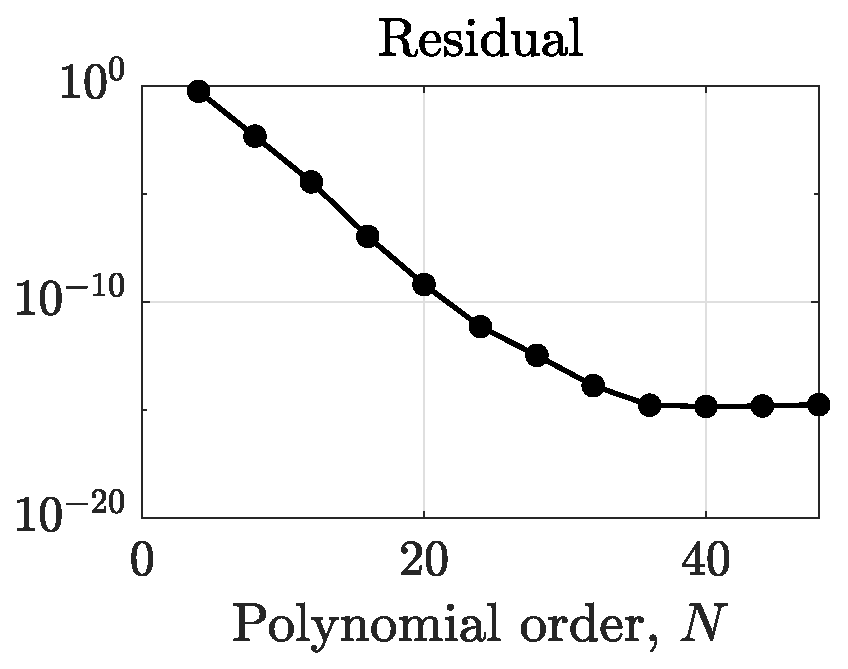
\includegraphics[height=0.3\linewidth]{Figures/moff_res}
\end{figure}

\end{frame}


\begin{frame}
\frametitle{Discontinuous boundary data: lid-driven cavity}
\centering
\begin{figure}
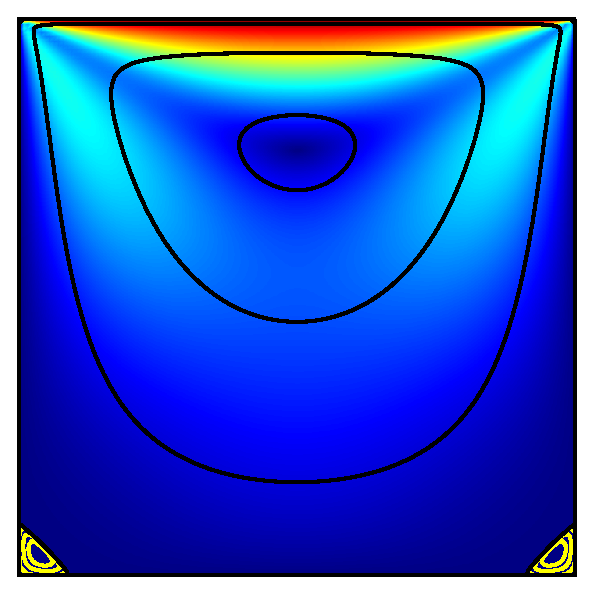
\includegraphics[height=0.5\linewidth]{Figures/ldc_soln}
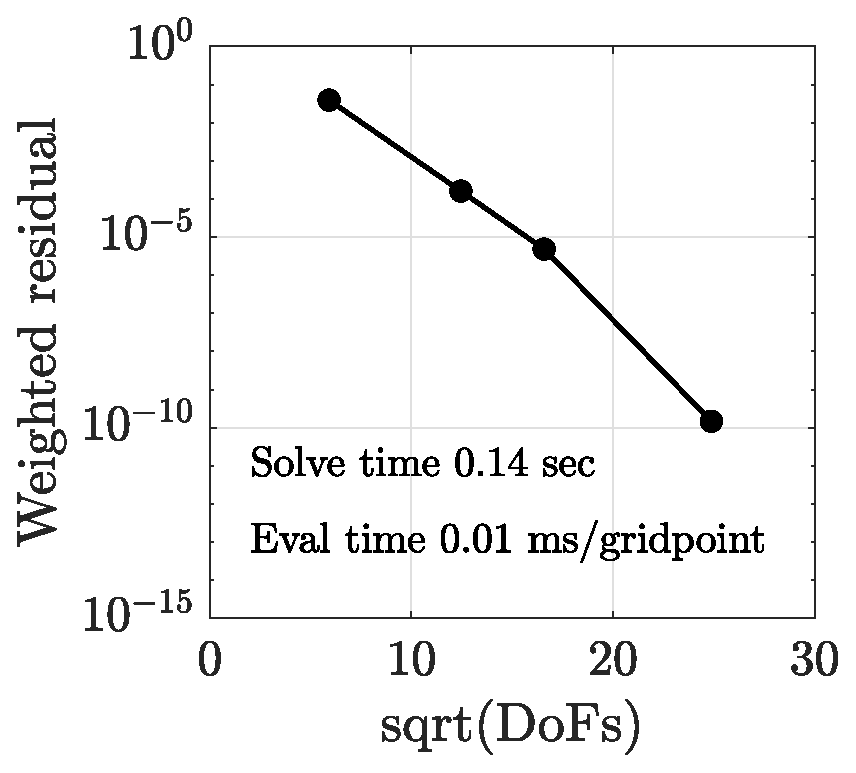
\includegraphics[height=0.4\linewidth]{Figures/ldc_conv}
\end{figure}
\end{frame}



\begin{frame}
\frametitle{Re-entrant corner: backwards-facing step}
\centering
\begin{figure}
	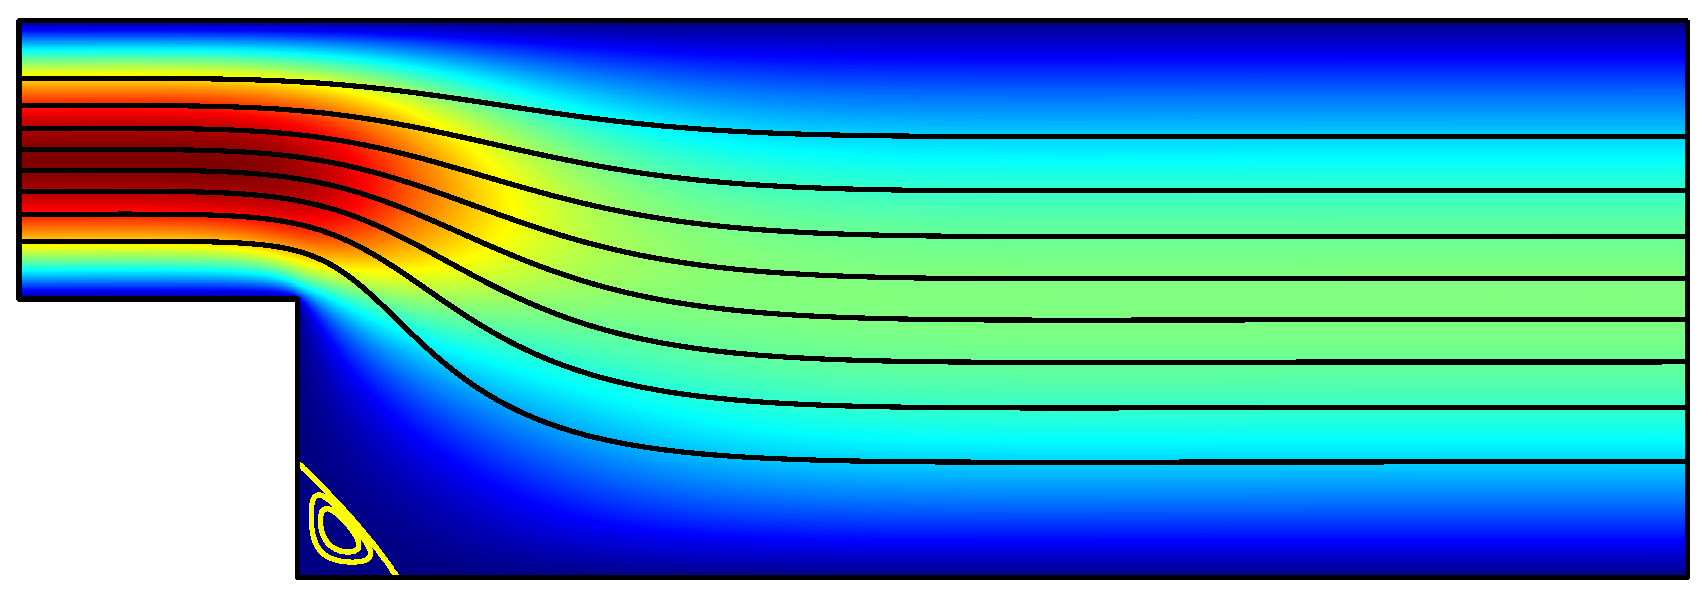
\includegraphics[height=0.3\linewidth]{Figures/step_soln}
	
	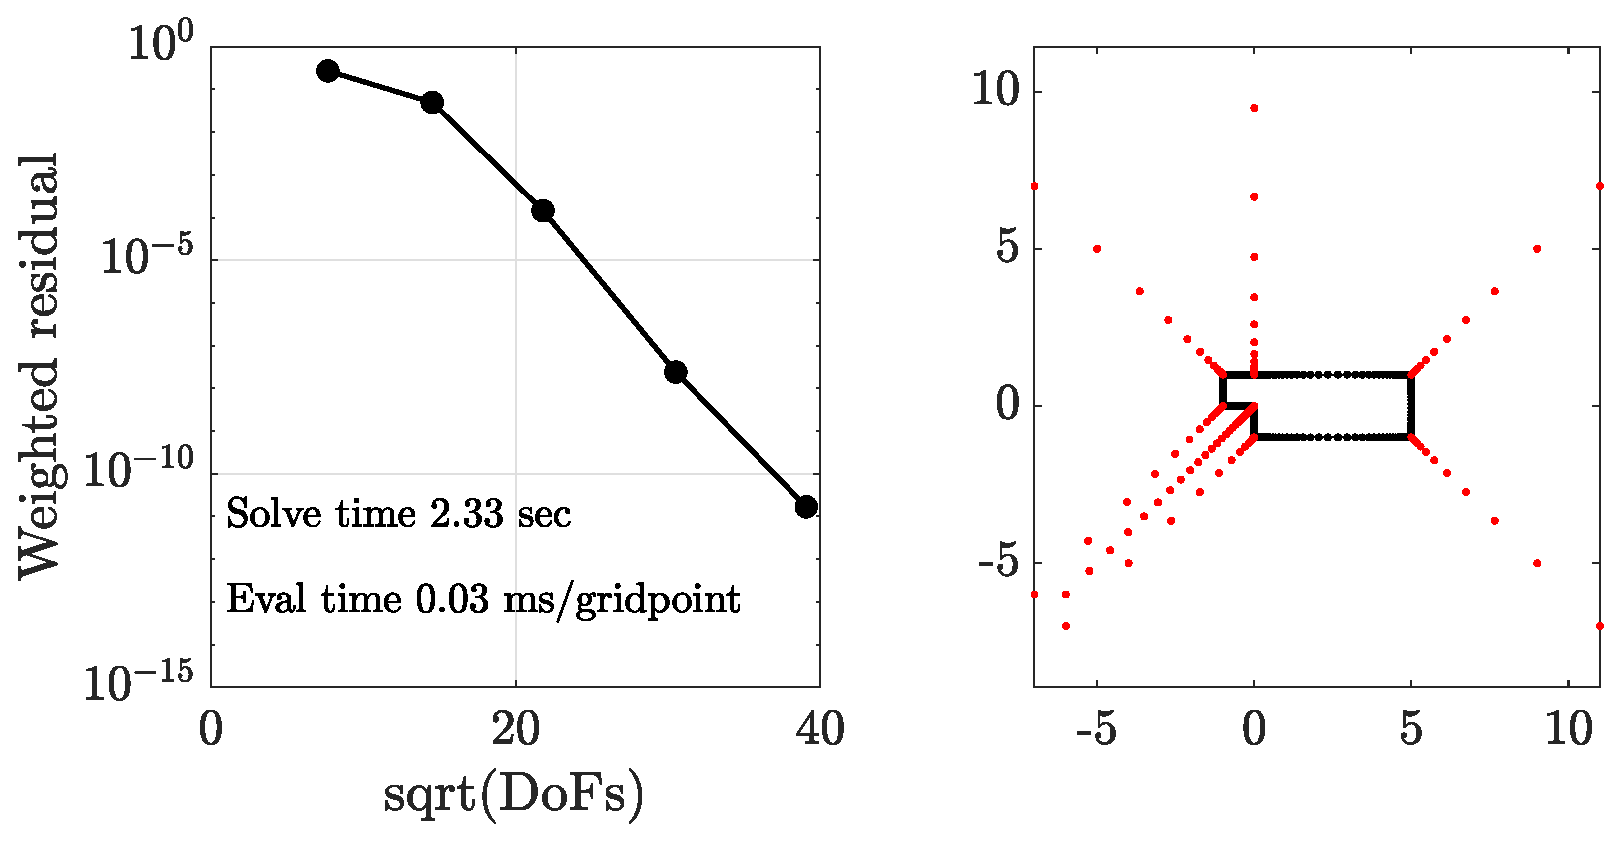
\includegraphics[height=0.3\linewidth]{Figures/step_conv}
\end{figure}
\end{frame}


\begin{frame}
\frametitle{The pressure and the velocity gradient blow up at the corner.}
\centering
\begin{figure}
	\includegraphics[width=\linewidth]{Figures/step_pres}
\end{figure}
\end{frame}


\begin{frame}
\frametitle{Infinitely long backwards-facing step}
\centering
\begin{figure}
	%\captionsetup{position=top}
	\subcaptionbox*{$-\infty\xleftarrow{\hspace*{0.4\linewidth}}x\xrightarrow{\hspace*{0.4\linewidth}}\infty$}{
		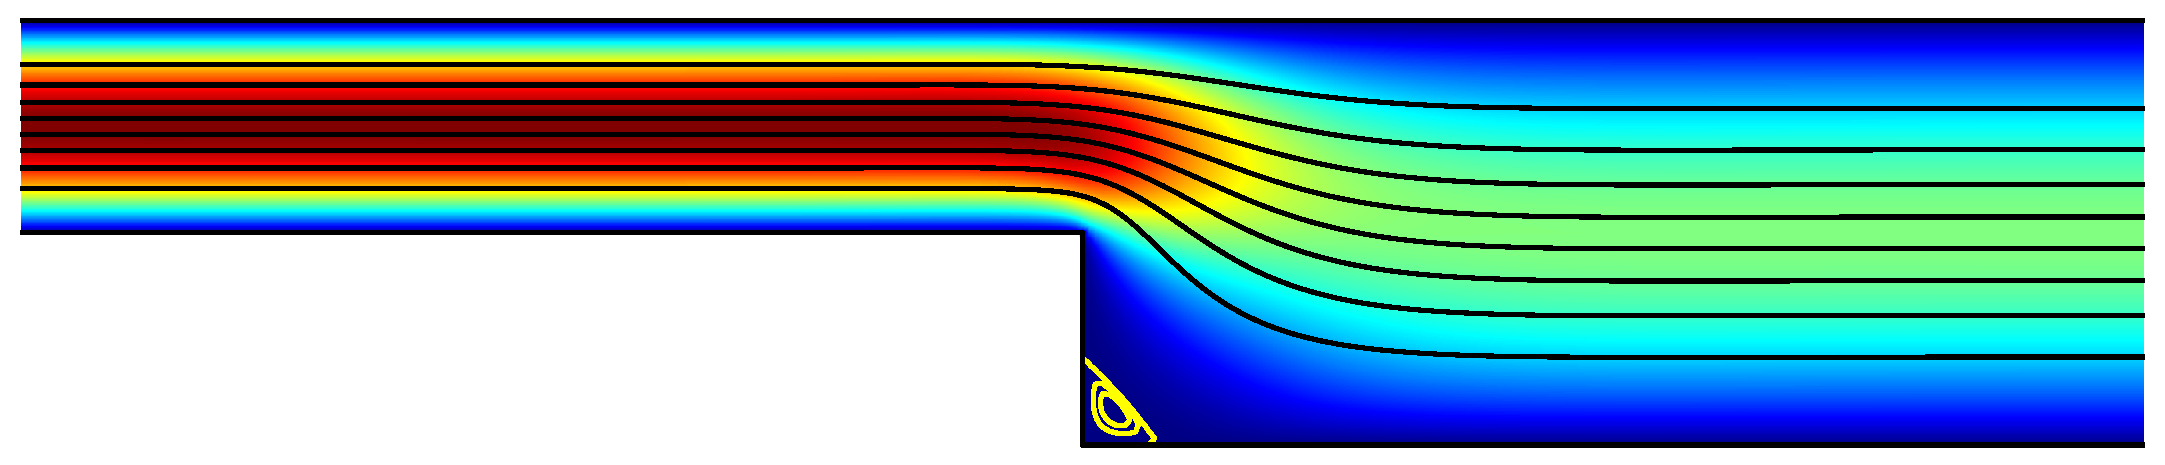
\includegraphics[width=\linewidth]{Figures/chan_soln}}
	\vfill
	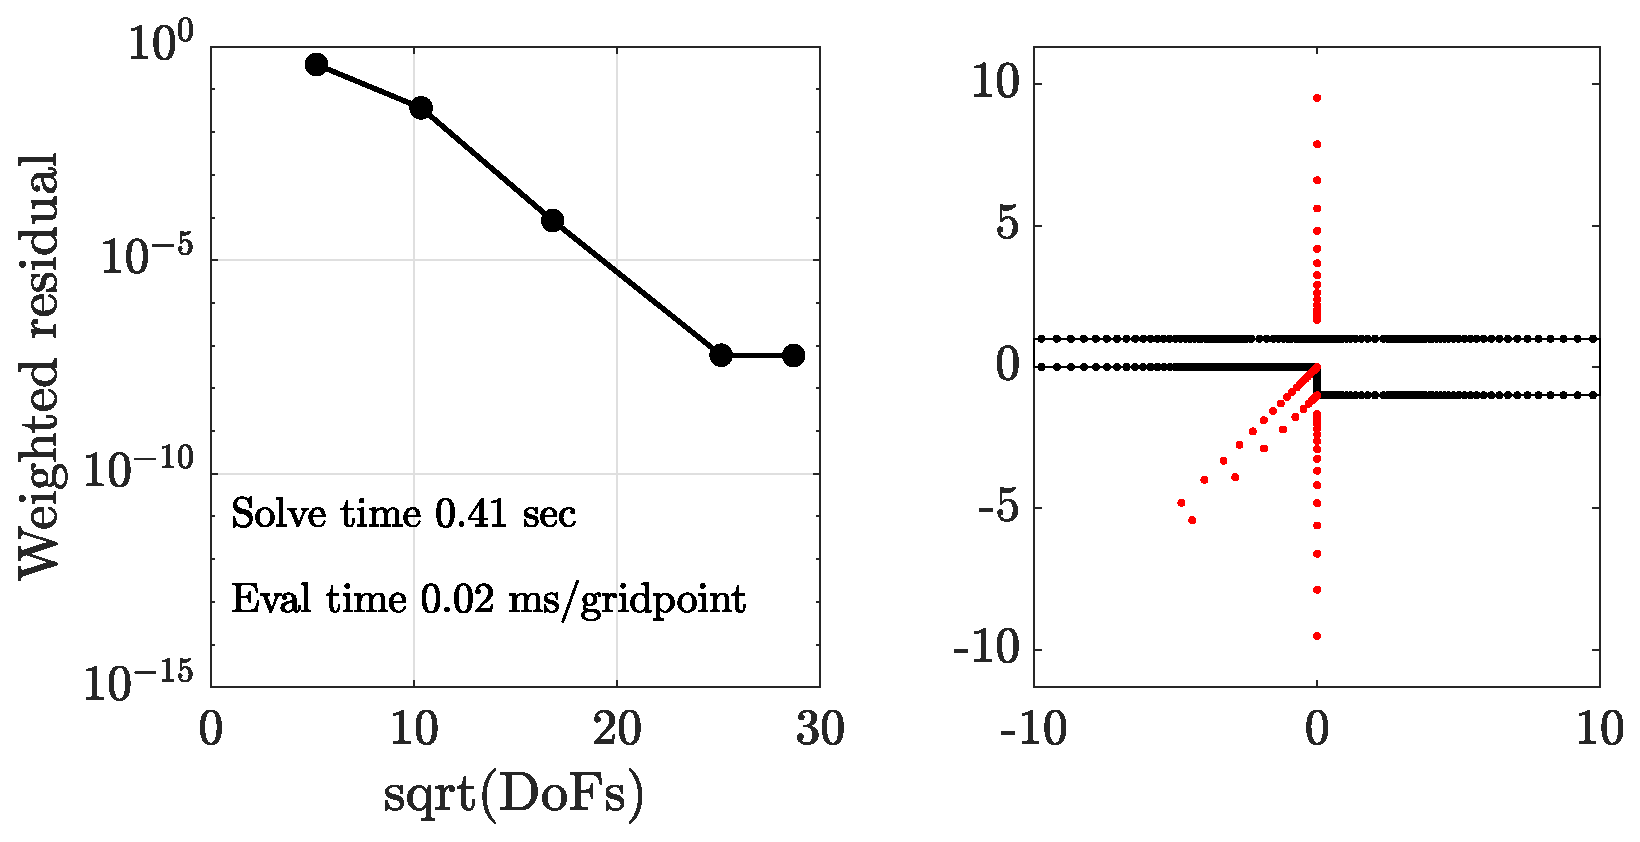
\includegraphics[height=0.3\linewidth]{Figures/chan_conv}
\end{figure}
\end{frame}


\begin{frame}
\frametitle{Infinite channel, flow past an obstacle}
\centering
\begin{figure}
	\subcaptionbox*{$-\infty\xleftarrow{\hspace*{0.4\linewidth}}x\xrightarrow{\hspace*{0.4\linewidth}}\infty$}{
	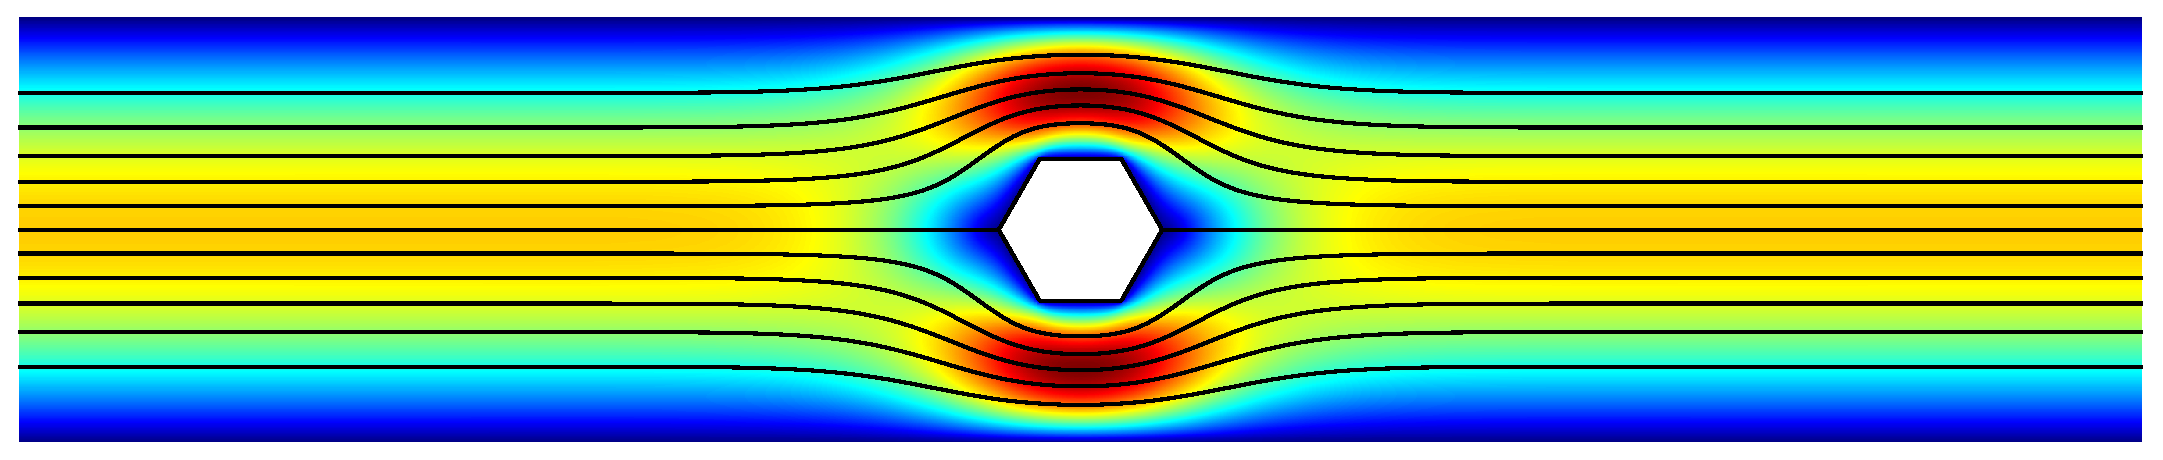
\includegraphics[width=\linewidth]{Figures/cyl_soln}}

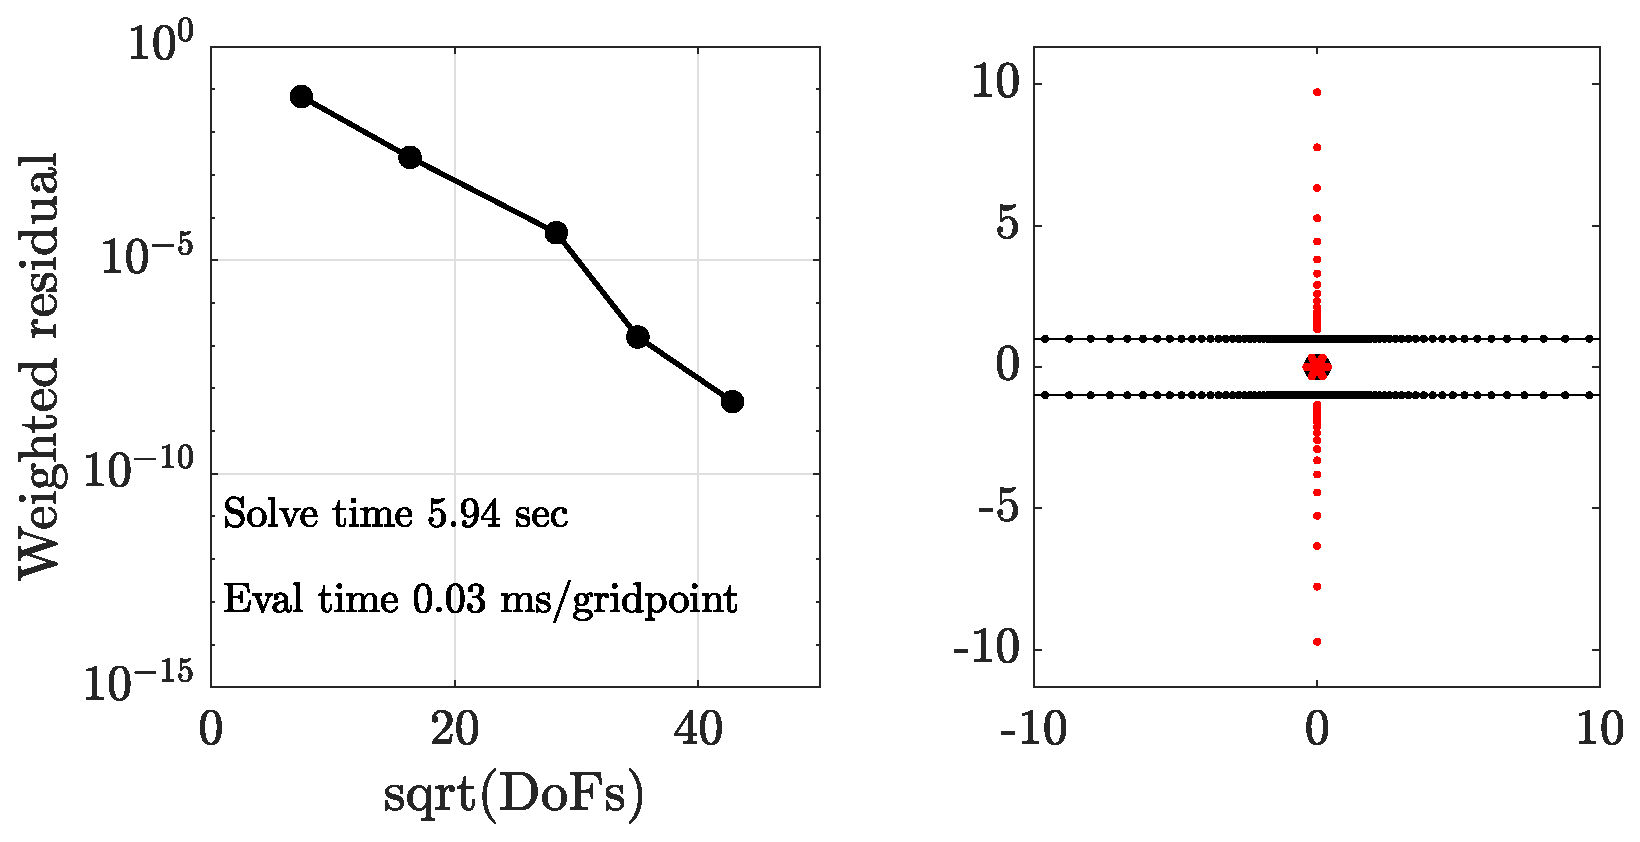
\includegraphics[height=0.3\linewidth]{Figures/cyl_conv}
\end{figure}
\end{frame}


\begin{frame}
\frametitle{Summary}
\begin{itemize}\itemsep 1em
\item Lightning Laplace for infinite and multiply connected regions
\item Lightning Stokes needs to solve for 2 analytic functions
\item Methods are computationally fast and converge root-exponentially
\end{itemize}

\bigskip
\textbf{Outlook}
\begin{itemize}\itemsep 1em
\item Multi-scale and domain decomposition approaches
\item Applications to linear elasticity
\end{itemize}

\end{frame}